\documentclass[12pt]{beamer}\usepackage[]{graphicx}\usepackage[]{color}
%% maxwidth is the original width if it is less than linewidth
%% otherwise use linewidth (to make sure the graphics do not exceed the margin)
\makeatletter
\def\maxwidth{ %
  \ifdim\Gin@nat@width>\linewidth
    \linewidth
  \else
    \Gin@nat@width
  \fi
}
\makeatother

\definecolor{fgcolor}{rgb}{0.345, 0.345, 0.345}
\newcommand{\hlnum}[1]{\textcolor[rgb]{0.686,0.059,0.569}{#1}}%
\newcommand{\hlstr}[1]{\textcolor[rgb]{0.192,0.494,0.8}{#1}}%
\newcommand{\hlcom}[1]{\textcolor[rgb]{0.678,0.584,0.686}{\textit{#1}}}%
\newcommand{\hlopt}[1]{\textcolor[rgb]{0,0,0}{#1}}%
\newcommand{\hlstd}[1]{\textcolor[rgb]{0.345,0.345,0.345}{#1}}%
\newcommand{\hlkwa}[1]{\textcolor[rgb]{0.161,0.373,0.58}{\textbf{#1}}}%
\newcommand{\hlkwb}[1]{\textcolor[rgb]{0.69,0.353,0.396}{#1}}%
\newcommand{\hlkwc}[1]{\textcolor[rgb]{0.333,0.667,0.333}{#1}}%
\newcommand{\hlkwd}[1]{\textcolor[rgb]{0.737,0.353,0.396}{\textbf{#1}}}%
\let\hlipl\hlkwb

\usepackage{framed}
\makeatletter
\newenvironment{kframe}{%
 \def\at@end@of@kframe{}%
 \ifinner\ifhmode%
  \def\at@end@of@kframe{\end{minipage}}%
  \begin{minipage}{\columnwidth}%
 \fi\fi%
 \def\FrameCommand##1{\hskip\@totalleftmargin \hskip-\fboxsep
 \colorbox{shadecolor}{##1}\hskip-\fboxsep
     % There is no \\@totalrightmargin, so:
     \hskip-\linewidth \hskip-\@totalleftmargin \hskip\columnwidth}%
 \MakeFramed {\advance\hsize-\width
   \@totalleftmargin\z@ \linewidth\hsize
   \@setminipage}}%
 {\par\unskip\endMakeFramed%
 \at@end@of@kframe}
\makeatother

\definecolor{shadecolor}{rgb}{.97, .97, .97}
\definecolor{messagecolor}{rgb}{0, 0, 0}
\definecolor{warningcolor}{rgb}{1, 0, 1}
\definecolor{errorcolor}{rgb}{1, 0, 0}
\newenvironment{knitrout}{}{} % an empty environment to be redefined in TeX

\usepackage{alltt}
\usepackage{tikz}

% make it pretty
% get rid of junk
\usetheme{default}
\usefonttheme[onlymath]{serif}
\beamertemplatenavigationsymbolsempty

% define a bunch of colors
\definecolor{offwhite}{RGB}{255,250,240}
\definecolor{gray}{RGB}{155,155,155}
\definecolor{foreground}{RGB}{80,80,80}
\definecolor{background}{RGB}{255,255,255}
%\definecolor{title}{RGB}{255,199,0}
\definecolor{title}{RGB}{89,132,212}
%\definecolor{subtitle}{RGB}{89,132,212}
\definecolor{subtitle}{RGB}{255,199,0}
\definecolor{hilit}{RGB}{248,117,79}
\definecolor{vhilit}{RGB}{255,111,207}
\definecolor{lolit}{RGB}{200,200,200}
\definecolor{lit}{RGB}{255,199,0}
\definecolor{mdlit}{RGB}{89,132,212}
\definecolor{link}{RGB}{248,117,79}

% a few color macros
\newcommand{\hilit}{\color{hilit}}
\newcommand{\vhilit}{\color{vhilit}}
\newcommand{\lit}{\color{lit}}
\newcommand{\mdlit}{\color{mdlit}}
\newcommand{\lolit}{\color{lolit}}

% use those colors
\setbeamercolor{titlelike}{fg=title}
\setbeamercolor{subtitle}{fg=subtitle}
\setbeamercolor{frametitle}{fg=gray}
%\setbeamercolor{structure}{fg=subtitle}
\setbeamercolor{structure}{fg=title}
\setbeamercolor{institute}{fg=lolit}
\setbeamercolor{normal text}{fg=foreground,bg=background}
\setbeamertemplate{itemize subitem}{{\textendash}}
\setbeamerfont{itemize/enumerate subbody}{size=\small}
\setbeamerfont{itemize/enumerate subitem}{size=\small}

% center title of slides
\setbeamertemplate{blocks}[rounded]
\setbeamertemplate{frametitle}[default][center]

% page number
\setbeamerfont{page number in foot}{size=\footnotesize}
\setbeamertemplate{footline}[frame number]

% default link color
\hypersetup{colorlinks, urlcolor={link}}

% a few macros
\newcommand{\code}[1]{\texttt{#1}}
\newcommand{\hicode}[1]{{\hilit \texttt{#1}}}
\newcommand{\locode}[1]{{\lolit \texttt{#1}}}
\newcommand{\bb}[1]{\begin{block}{#1}}
\newcommand{\eb}{\end{block}}
\newcommand{\bi}{\begin{itemize}}
\newcommand{\bbi}{\vspace{4pt} \begin{itemize} \itemsep8pt}
\newcommand{\ei}{\end{itemize}}
\newcommand{\bv}{\begin{verbatim}}
\newcommand{\ev}{\end{verbatim}}
\newcommand{\ig}{\includegraphics}
\newcommand{\subt}[1]{{\footnotesize \color{subtitle} {#1}}}
\newcommand{\ttsm}{\tt \small}
\newcommand{\ttfn}{\tt \footnotesize}
\newcommand{\figh}[2]{\centerline{\includegraphics[height=#2\textheight]{#1}}}
\newcommand{\figw}[2]{\centerline{\includegraphics[width=#2\textwidth]{#1}}}



%------------------------------------------------

\title{Power Method}
\subtitle{Matrix Algebra 4 Statistical Learning}
\author{\href{http://www.gastonsanchez.com}{Gaston Sanchez}}
\institute{\href{https://creativecommons.org/licenses/by-sa/4.0/}{\tt \scriptsize \color{foreground} CC BY-SA 4.0}}
\date{}
\IfFileExists{upquote.sty}{\usepackage{upquote}}{}
\begin{document}



% no page number in first slide
{
  \setbeamertemplate{footline}{} 
  \frame{\titlepage} 
}

%------------------------------------------------

\begin{frame}
\begin{center}
\Huge{\hilit{Power Method}}
\end{center}
\end{frame}

%------------------------------------------------

\begin{frame}
\frametitle{About the Power Method}

One of the basic procedures following a successive approximation 
approach for the dominant eigenvector is precisely the {\hilit Power Method}.

\bigskip
In its simplest form, the Power Method (PM) allows us to find \textbf{the largest} 
eigenvector and its corresponding eigenvalue.

\end{frame}

%------------------------------------------------

\begin{frame}
\frametitle{About the Power Method}

Choose an arbitrary vector $\mathbf{w_0}$ to which we will apply the symmetric matrix 
$\mathbf{S}$ repeatedly to form the following sequence:

\begin{align*}
 \mathbf{w_1} &= \mathbf{S w_0} \\
 \mathbf{w_2} &= \mathbf{S w_1 = S^2 w_0} \\
 \mathbf{w_3} &= \mathbf{S w_2 = S^3 w_0} \\
 \vdots \\
 \mathbf{w_k} &= \mathbf{S w_{k-1} = S^k w_0}
\end{align*}

\end{frame}

%------------------------------------------------

\begin{frame}[fragile]
\frametitle{Power Method: Example}

Consider a matrix $\mathbf{S}$
$$
\mathbf{S} =
\begin{bmatrix}
3 & 1 \\
1 & 2 \\
\end{bmatrix}
$$

\bigskip
and an initial vector $\mathbf{w_0}$
$$
\mathbf{w_0} =
\begin{bmatrix}
-0.4 \\
1.3 \\
\end{bmatrix}
$$

\end{frame}

%------------------------------------------------

\begin{frame}[fragile]

\begin{knitrout}\footnotesize
\definecolor{shadecolor}{rgb}{0.969, 0.969, 0.969}\color{fgcolor}

{\centering 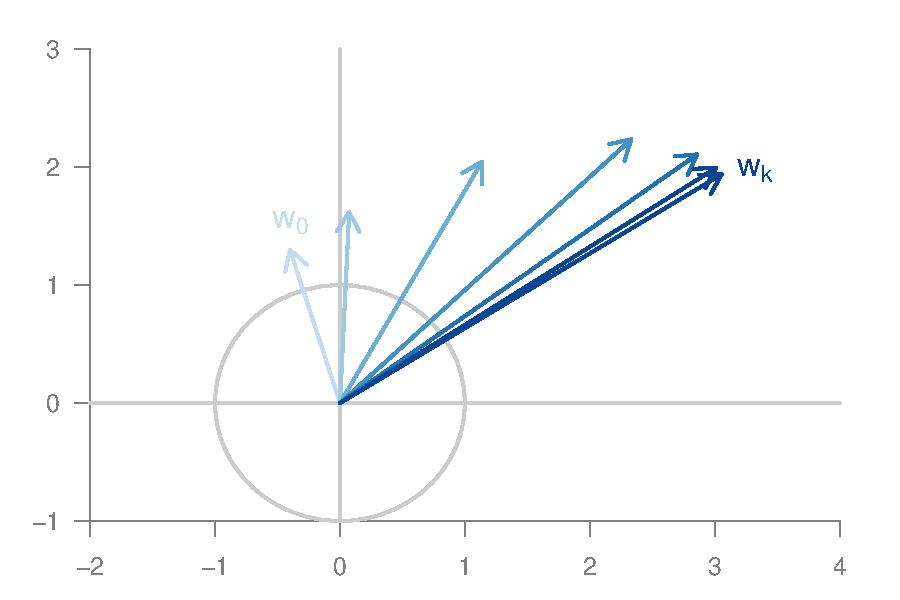
\includegraphics[width=\maxwidth]{figure/power-method-example-1} 

}



\end{knitrout}

\end{frame}

%------------------------------------------------

\begin{frame}
\frametitle{About the Power Method}

\bbi
  \item In practice, we must rescale the obtained vector $\mathbf{w_k}$ at each step.
  \item The rescaling will allows us to judge whether the sequence is converging.
  \item After some iterations, the vector $\mathbf{w_{k-1}}$ and $\mathbf{w_k}$ will be very similar
  \item Assuming a reasonable scaling strategy, the sequence will usually converge 
  to the dominant eigenvector of $\mathbf{S}$.
\ei

\end{frame}

%------------------------------------------------

\begin{frame}[fragile]

\begin{knitrout}\footnotesize
\definecolor{shadecolor}{rgb}{0.969, 0.969, 0.969}\color{fgcolor}

{\centering 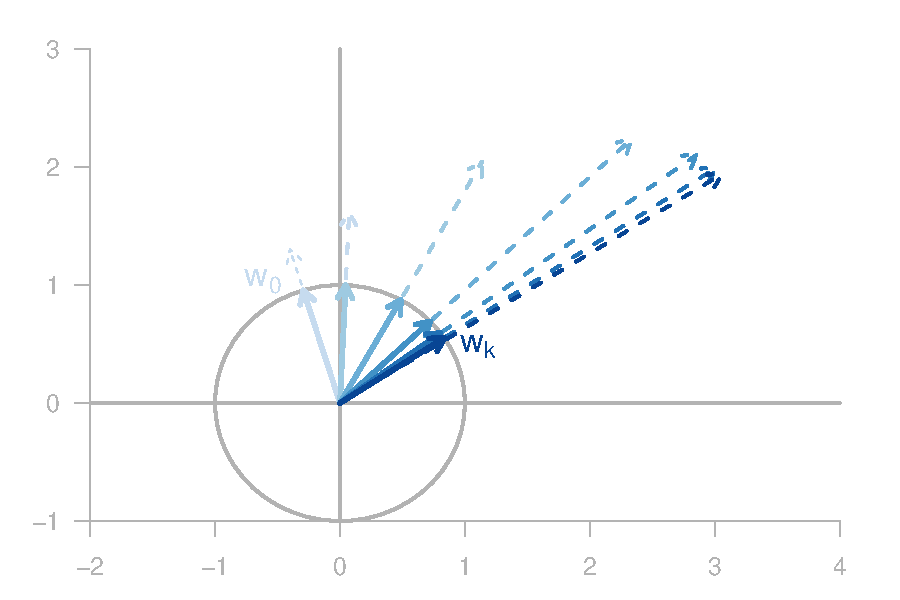
\includegraphics[width=\maxwidth]{figure/power-method-rescale-1} 

}



\end{knitrout}

\end{frame}

%------------------------------------------------

\begin{frame}
\frametitle{Dominant Eigenvalue}

The obtained vector is the dominant eigenvector. To get the 
corresponding eigenvalue we calculate the so-called \textbf{Rayleigh quotient}
given by:

{\Large
$$
\lambda = \frac{\mathbf{w_{k}^{\mathsf{T}} S w_k}}{\mathbf{w_{k}^{\mathsf{T}} w_k}}
$$
}

\end{frame}

%------------------------------------------------

\begin{frame}
\frametitle{Remarks}

Conditions for the power method to be succesfully used: 
\bbi
  \item The matrix must have a \textit{dominant} eigenvalue. 
  \item The starting vector $\mathbf{w_0}$ must be nonzero. 
  \item We need to scale each of the vectors $\mathbf{w_k}$ \\
  {\lolit otherwise the algorithm will ``explode''}
\ei

\end{frame}

%------------------------------------------------

\begin{frame}
\frametitle{PM Pseudocode}

Let's consider a more detailed version of the PM algorithm:
\begin{enumerate}
  \item Start with an arbitraty initial vector $\mathbf{w}$
  \item Obtain product $\mathbf{\tilde{w} = S w}$
  \item Normalize $\mathbf{\tilde{w}}$
  $$
  \text{e.g.} \quad \mathbf{w} = \frac{\mathbf{\tilde{w}}}{\| \mathbf{\tilde{w}} \|_{p=2}}
  $$
  \item Compare $\mathbf{w}$ with its previous version
  \item Repeat steps 2 till 4 until convergence
\end{enumerate}

\end{frame}

%------------------------------------------------

\begin{frame}
\frametitle{Why does the PM work?}

Assume that the matrix $\mathbf{S}$ has $p$ eigenvalues 
$\lambda_1, \lambda_2, \dots, \lambda_p$, and that they are ordered in 
decreasing way $|\lambda_1| > |\lambda_2| \geq \dots \geq |\lambda_p|$.

\bigskip
Note that the first eigenvalue is strictly greater than the second one. This is 
a very important assumption.

\bigskip
In the same way, we'll assume that the matrix $\mathbf{S}$ has $p$ linearly 
independent vectors $\mathbf{u_1}, \dots, \mathbf{u_p}$ ordered in such a way 
that $\mathbf{u_j}$ corresponds to $\lambda_j$. 

\end{frame}

%------------------------------------------------

\begin{frame}
\frametitle{Why does the PM work?}

The initial vector $\mathbf{w_0}$ may be expressed as a linear combination of 
$\mathbf{u_1}, \dots, \mathbf{u_p}$

$$
\mathbf{w_0} = a_1 \mathbf{u_1} + \dots + a_p \mathbf{u_p}
$$

At every step of the iterative process the vector $\mathbf{w_k}$ is given by:

$$
\mathbf{w_k} = a_1 \lambda_{1}^k \mathbf{u_1} + \dots + a_p \lambda_{p}^k \mathbf{u_p}
$$

\end{frame}

%------------------------------------------------

\begin{frame}
\frametitle{Why does the PM work?}

Since $\lambda_1$ is the dominant eigenvalue, the component in the direction of 
$\mathbf{u_1}$ becomes relatively greater than the other components as $k$ 
increases. If we knew $\lambda_1$ in advance, we could rescale at each step by 
dividing by it to get:

$$
\left(\frac{1}{\lambda_{1}^k}\right) \mathbf{w_k}= a_1 \mathbf{u_1} + \dots + a_p \left(\frac{\lambda_{p}^k}{\lambda_{1}^k}\right) \mathbf{u_p}
$$

which converges to the eigenvector $a_1 \mathbf{u_1}$, provided that $a_1$ is nonzero.

\end{frame}

%------------------------------------------------

\begin{frame}
\frametitle{Why does the PM work?}

Of course, in real life this scaling strategy is not possible---we 
don't know $\lambda_1$. Consequenlty, the eigenvector is determined only up to 
a constant multiple, which is not a concern since the really important thing is 
the \textit{direction} not the length of the vector.

\bigskip
The speed of the convergence depends on how bigger $\lambda_1$ is respect with 
to $\lambda_2$, and on the choice of the initial vector $\mathbf{w_0}$. If 
$\lambda_1$ is not much larger than $\lambda_2$, then the convergence will be 
slow.

\end{frame}

%------------------------------------------------

\begin{frame}
\frametitle{More Remarks}

\bbi
  \item The power method is a sequential method.
  \item We can obtain $\mathbf{w_1, w_2}$, and so on, step by step.
  \item If we only need the first $k$ vectors, we can stop the procedure at the desired stage.
\ei

\end{frame}

%------------------------------------------------

\begin{frame}
\frametitle{Obtaining more eigenvectors?}

For \textbf{symmetric} matrices, once we've obtained the first eigenvector 
$\mathbf{w_1}$ and eigenvalue $\lambda_1$, we can compute the second eigenvector 
by reducing the matrix $\mathbf{S}$ by the 
amount explained by the first eigenvector. 

\bigskip
This operation of reduction is called \textbf{deflation} 
and the residual matrix is obtained as:

{\large
$$
\mathbf{S_1} = \mathbf{S} - \lambda_1 \mathbf{w_1 w_{1}^\mathsf{T}}
$$
}

To get the second eigenvalue and its corresponding eigenvector, 
we operate on $\mathbf{S_1}$ in the same way as the operations on $\mathbf{S}$.

\end{frame}

%------------------------------------------------

\begin{frame}
\frametitle{Bibliography}

{\footnotesize
\bi
  \item \textbf{Multivariate Analysis} by Maurice Tatsuoka (1988).
  \textit{Chapter 5: More Matrix Algebra}. Macmillan Publishing.
  \item \textbf{Mathematical Tools for Applied Multivariate Analysis} by J.D. Carroll, P.E. Green, and A. Chaturvedi (1997). 
  \textit{Chapter 5: Decomposition of Matrix Transformations: Eigenstructures and Quadratic Forms}. Academic Press. 
  \item \textbf{Hands-on Matrix Algebra using R} by Hrishikesh Vinod (2011).
  \textit{Chapter 9: Eigenvalues and Eigenvectors}. World Scientific.
\ei
}

\end{frame}

%------------------------------------------------

\end{document}
